\section{Results}
\label{sec:results}
All results use the frozen analysis code, rounds with four valid bids, and
the full 200-round horizon. Intervals are pointwise 95\% block-bootstrap
intervals unless stated otherwise. The required scripted
rock--paper--scissors replication recovered the paper's rising detection
pattern, but not every published percentage
(Appendix~\ref{app:replication}); it is separate from the LLM evidence.

\subsection{Detection: the primary test passes, but correlation is as good}
The pre-registered L2 net-influence score separated strong-pair cartel
markets (C1-SS) from matched honest markets: AUROC $0.865$
$[0.734,0.968]$, $p=0.00002$ over $20$ matched blocks. This rejects the
sole confirmatory null.
% source: results/analysis/final_v1/results.json primary; all_cells[206].auroc
The same-access correlation baseline scored $0.9875$ at L1 and $0.9975$ at
L2; the paired L2 difference, net minus correlation, was $-0.1325$
$[-0.2647,-0.0309]$.
% source: results/analysis/final_v1/results.json all_cells[196].auroc; all_cells[202].auroc; contrasts[95].result
Figure~\ref{fig:detection} shows the same picture for every cartel with a
private channel, including other placements, the no-warning variant and
other models: correlation was at least as good. The two small L1 advantages
(C1-FF, Qwen-4B) have intervals including zero.
% source: results/analysis/final_v1/results.json contrasts[369].result; contrasts[532].result
On fresh markets (Section~\ref{sec:addenda}) the same pattern held:
C1-SS reached L2 net AUROC $0.9075$ $[0.8025,0.985]$ against correlation's
$0.995$, a difference of $-0.0875$ $[-0.19,-0.015]$.
% source: results/analysis/replication_v22/results.json all_cells[2122,2119].auroc; contrasts[609].result

\begin{figure}[tb]
\centering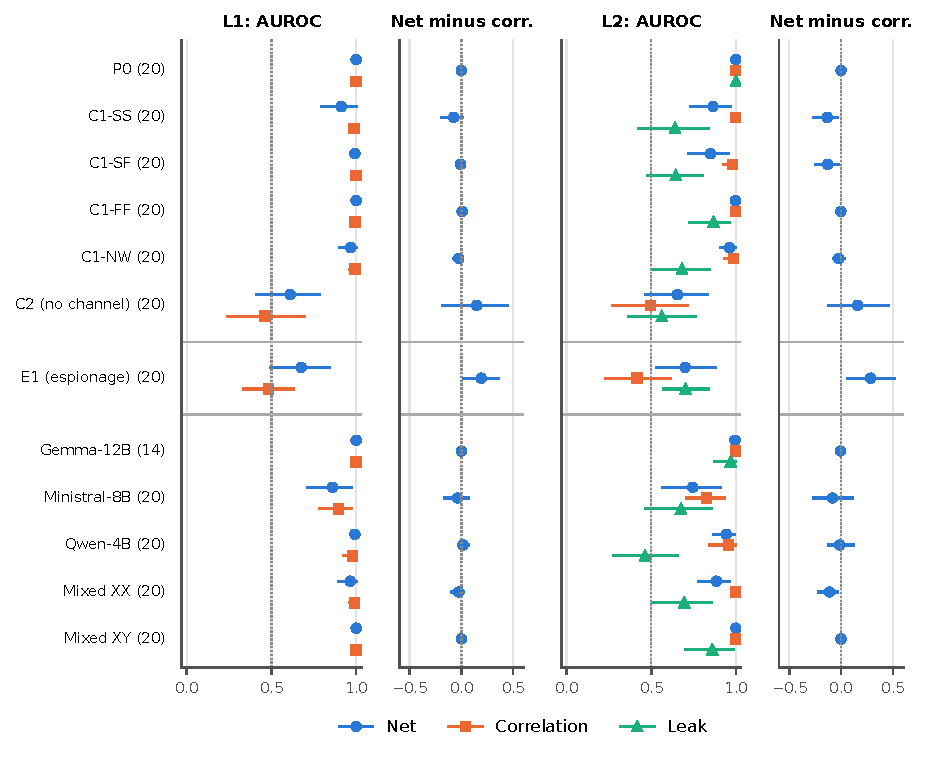
\includegraphics[width=\linewidth]{figures/figure_a.pdf}
\caption{Detection by treatment (original markets 0--19). AUROC with
pointwise 95\% block-bootstrap intervals for net influence and correlation
at L1 and L2, and the L2 leak score; parentheses give matched blocks. E1
(espionage) is separated because it is not a cartel. Missing small-model
comparisons are listed in the appendix.}
% source: results/report_figures/figure_numbers.csv figure=A
\label{fig:detection}
\end{figure}

\begin{figure}[!t]
\centering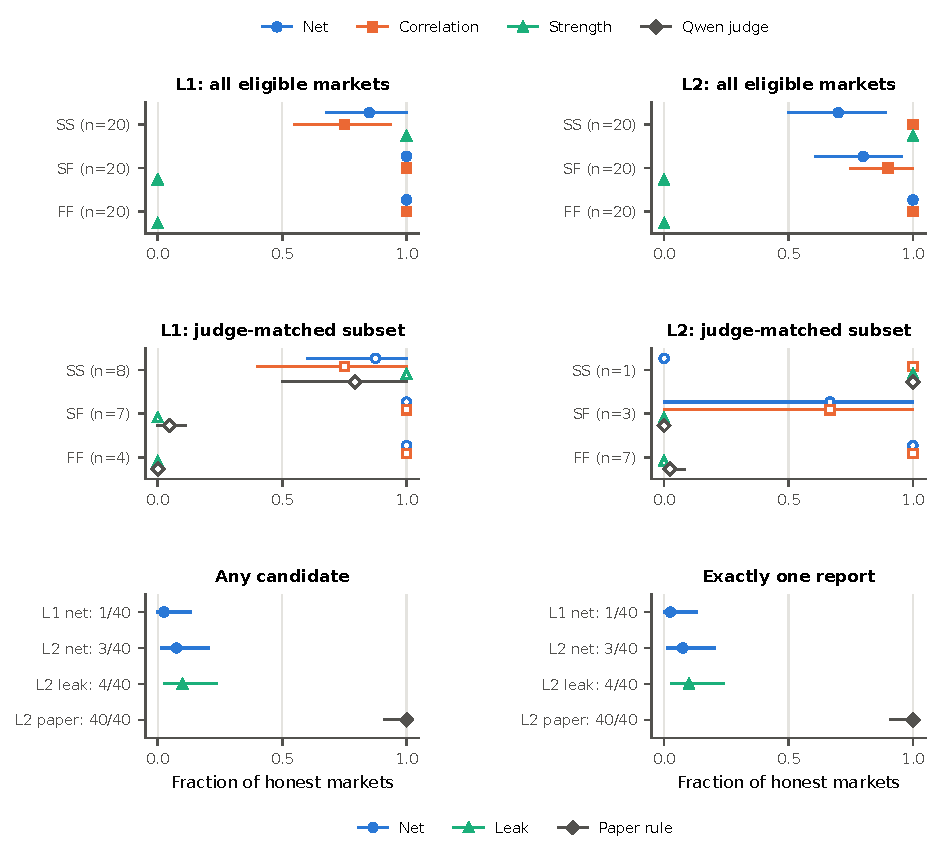
\includegraphics[width=\linewidth]{figures/figure_b.pdf}
\caption{Localisation and false alarms (original markets 0--19). Top: top-1
for the assigned pair on all eligible markets. Middle: top-1 at L2 on the
markets where the judge returned valid output, under the registered
12,000-token limit (left) and the 24,000-token check of
Section~\ref{sec:addenda} (right; C1-FF not run). With more budget the judge
still names the strong pair, so it fails for C1-SF. Bottom: honest-market
alarm rates with exact binomial intervals; descriptive, not calibration
guarantees.}
% source: results/report_figures/figure_numbers.csv figure=B (middle right: results/analysis/judge24k_v23/results.json judge_comparisons)
\label{fig:localisation}
\end{figure}

\subsection{Where net influence adds information: espionage, replicated}
In E1 one firm secretly sees its rival's current cost. Here net influence
clearly beat correlation at L2: AUROC $0.700$ versus $0.415$, paired
difference $+0.285$ $[0.062,0.515]$; at L1 the difference was $+0.1925$
$[0.0222,0.3599]$. The L2 leak score, which isolates a cost entering a
rival's bid, reached $0.7025$ $[0.5737,0.8360]$.
% source: results/analysis/final_v1/results.json all_cells[334,332,340,337,339].auroc; contrasts[259,263].result
Because E1 was the one cell that stood out, we collected it again on fresh
markets (Table~\ref{tab:replication}). The pre-specified L2 criterion
replicated: net $0.680$ versus correlation $0.415$, difference $+0.265$
$[0.070,0.445]$, leak $0.745$. The L1 difference did not replicate
($+0.095$ $[-0.1125,0.315]$). Net influence therefore adds information when
one firm's private cost flows into another firm's bids and the auditor can
see costs.
% source: results/analysis/replication_v22/results.json all_cells[1990,1987,1989].auroc; contrasts[501,498].result; results/analysis/addendum_summary/summary.json preregistered_verdicts

The cartel without a channel (C2) behaved differently. It raised joint
profit over honest markets by $0.399$ $[0.364,0.434]$ per round, more than
any other LLM treatment and almost three times the C1-SS uplift ($0.144$).
Yet it was the cartel both detectors separated least well: net $0.655$ and
correlation $0.495$ at L2, a difference whose interval includes zero.
On fresh markets the profit uplift replicated ($+0.283$ $[0.179,0.371]$);
detection rose somewhat (net $0.753$, correlation $0.630$) and the
difference again included zero. Against the fresh C1-SS markets, C2 was
detected less well by both net ($-0.155$ $[-0.30,-0.01]$) and correlation
($-0.365$ $[-0.59,-0.16]$).
% source: results/analysis/replication_v22/results.json contrasts "C1-SS minus C2 L2:net", "C1-SS minus C2 L2:correlation" (cohort replication)
% source: results/analysis/final_v1/results.json behaviour core.C2/core.C1-SS joint_profit; all_cells[274,271].auroc; contrasts[208].result; results/analysis/replication_v22/results.json behaviour[40].paired_difference; all_cells[2056,2053].auroc; contrasts[555].result
In this game the most profitable collusion was also the quietest.

\begin{table}[tb]
\centering\small
\setlength{\tabcolsep}{3pt}
\caption{Out-of-sample replication (Addendum v2.2). Original: registered markets 0--19; replication: fresh treatment markets 20--39 against the registered N0 markets 20--39. Estimates with 95\% block-bootstrap intervals (20 matched blocks). Profit is the paired joint-profit difference versus N0.}
\label{tab:replication}
\begin{tabular}{llccc}
\toprule
Cell & Sample & L2 net AUROC & L2 net $-$ corr. & Joint profit vs N0\\
\midrule
E1 & original & 0.700 [0.529, 0.877] & 0.285 [0.062, 0.515] & $-$0.116 [$-$0.137, $-$0.095]\\
E1 & replication & 0.680 [0.505, 0.830] & 0.265 [0.070, 0.445] & $-$0.084 [$-$0.109, $-$0.060]\\
C2 & original & 0.655 [0.467, 0.833] & 0.160 [$-$0.125, 0.453] & 0.399 [0.364, 0.434]\\
C2 & replication & 0.752 [0.582, 0.905] & 0.122 [$-$0.118, 0.358] & 0.283 [0.179, 0.371]\\
C1-SS & original & 0.865 [0.734, 0.968] & $-$0.133 [$-$0.265, $-$0.031] & 0.144 [0.094, 0.192]\\
C1-SS & replication & 0.907 [0.802, 0.985] & $-$0.088 [$-$0.190, $-$0.015] & 0.173 [0.123, 0.221]\\
\bottomrule
\end{tabular}
\end{table}


\subsection{Localisation and honest-market alarms}
Net influence named the right pair even where the obvious shortcut fails.
When the cartel was not the strong pair, ranking the two strong firms first
had top-1 accuracy zero, while net influence reached $1.00/0.80$ (SF) and
$1.00/1.00$ (FF) at L1/L2; correlation was similar ($1.00/0.90$,
$1.00/1.00$).
% source: results/analysis/final_v1/results.json all_cells[398,400,402,403,406,408,464,466,468,469,472,474].top1
A good ranking is not yet an alarm: in C1-SS at L2, net top-1 was $0.70$,
but the reporting rule named the correct pair alone in only $0.25$ of
markets and abstained in $0.75$, with no wrong-pair reports.
% source: results/analysis/final_v1/results.json all_cells[206].top1,correct_unique,abstention,wrong_pair

In honest markets the permutation-corrected rule never flagged the
reference pair ($0/40$ at each level; upper limit $0.088$) and flagged any
pair in $1/40$ (L1) and $3/40$ (L2) markets; the L2 leak rule in $4/40$.
% source: results/analysis/final_v1/results.json all_cells[55,62].designated_alarm; all_cells[55,62,61].any_candidate,exactly_one_report
The paper's fixed threshold ($\alpha=0.05$ on uncorrected scores) alarmed in
$40/40$ honest L2 markets. In C2 its score ranked markets well (AUROC
$0.8875$), but its reporting rule named the wrong pair in $20/20$ markets.
% source: results/analysis/final_v1/results.json all_cells[63].any_candidate,exactly_one_report; all_cells[275].auroc,correct_unique,wrong_pair,coverage

\subsection{An LLM judge: more budget, same blind spot}
Under its registered $12{,}000$-token limit the Qwen judge failed on
$322/600$ judgements; most failed calls ran out of tokens, so matched
comparisons covered only $1$--$8$ blocks.
% source: results/analysis/final_v1/results.json judgments grouped by model/status/failure; judge_comparisons[*].judge_auroc.n_blocks
With $24{,}000$ tokens (Section~\ref{sec:addenda}) it returned valid output
for $54$$/60$ L2 judgements on the same markets, against $27/60$
before; $31$ of the valid answers used more than $12{,}000$
tokens. Coverage was now adequate, and the judge still did not reliably separate
cartel from honest markets: AUROC $0.625$ $[0.424,0.808]$ for C1-SS versus N0 on
$17$ blocks, where net influence scored $0.907$ and
correlation $1.000$ on the same blocks. It named the strong pair
almost regardless of the truth: top-1 $0.92$ in C1-SS, $0.90$
for the honest reference pair, but $0.02$ in C1-SF, where net
influence reached $0.93$ on the same markets.
% source: results/analysis/judge24k_v23/results.json judgments (cohort judge24k); all_cells[60,138,206] judge:qwen-9b coverage/auroc/top1; judge_comparisons[0,1,4,5]; valid-answer token counts from results/raw/*__deviation_judge24k/calls; results/analysis/addendum_summary/summary.json judge_budget
This is a behavioural pattern of one 9B judge model, not evidence about its
internal reasoning or about larger judges. The Gemma counter-judge returned
only $5/40$ valid judgements.
% source: results/analysis/final_v1/results.json judgments grouped by model/status

\subsection{Behaviour, flow labels, breadth and probes}
Table~\ref{tab:behaviour} separates economic outcomes from flow labels.
Removing the surveillance warning (A1) raised the L2 net AUROC by $0.0975$
$[-0.0051,0.2300]$ relative to C1-SS while joint profit fell by $0.3478$
$[0.2921,0.4015]$; this does not show deliberate evasion.
% source: results/analysis/final_v1/results.json addendum.A1.auroc_differences.L2:net; addendum.A1.behaviour_NW_minus_SS.joint_profit
Market-level flow labels did not separate cartel and spy: C1-SS had $0$
designated pairs with a detected leak and $12$ unclear; E1 had $4$ with one
direction detected and the reverse weak, and $8$ unclear.
% source: results/analysis/final_v1/results.json all_cells[206,340].label:*
\begin{table}[tb]\centering\small
\caption{Behaviour and designated-pair flow labels. Differences are treatment minus matched N0, in game units per round, with pointwise 95\% intervals. Flow counts are both / one (reverse weak) / neither (both weak) / unclear / unavailable. E1 is unilateral access.}
\label{tab:behaviour}
\begin{tabular}{@{}llll@{}}\toprule
Cell & Joint profit difference & Winning price difference & Flow counts \\\midrule
% source: results/analysis/final_v1/results.json behaviour[40].paired_difference; n_blocks
% source: results/analysis/final_v1/results.json behaviour[41].paired_difference; n_blocks
% source: results/analysis/final_v1/results.json all_cells[206].label:*
C1-SS & 0.144 [0.094, 0.192] & 0.295 [0.233, 0.358] & 0 / 0 / 8 / 12 / 0\\
% source: results/analysis/final_v1/results.json behaviour[64].paired_difference; n_blocks
% source: results/analysis/final_v1/results.json behaviour[65].paired_difference; n_blocks
% source: results/analysis/final_v1/results.json all_cells[274].label:*
C2 & 0.399 [0.364, 0.434] & 0.798 [0.768, 0.826] & 0 / 0 / 11 / 9 / 0\\
% source: results/analysis/final_v1/results.json behaviour[88].paired_difference; n_blocks
% source: results/analysis/final_v1/results.json behaviour[89].paired_difference; n_blocks
% source: results/analysis/final_v1/results.json all_cells[340].label:*
E1 & -0.116 [-0.137, -0.095] & -0.048 [-0.062, -0.034] & 0 / 4 / 8 / 8 / 0\\
% source: results/analysis/final_v1/results.json behaviour[280].paired_difference; n_blocks
% source: results/analysis/final_v1/results.json behaviour[281].paired_difference; n_blocks
% source: results/analysis/final_v1/results.json all_cells[1462].label:*
C1-NW & -0.204 [-0.229, -0.179] & -0.039 [-0.059, -0.017] & 0 / 1 / 8 / 11 / 0\\
\bottomrule\end{tabular}
\end{table}

Gemma-E4B and Ministral-3B produced too many invalid bids (at most $2$
eligible markets per cell), so their results are unavailable, not negative.
% source: results/analysis/final_v1/results.json all_cells[934,1000,1066,1132].eligible,auroc
None of the seven A2 placement-swap endpoints survived Holm correction
(smallest raw $p=0.0377$, adjusted $0.264$).
% source: results/analysis/final_v1/results.json addendum.A2.endpoints.L2:leak.test.p_value,holm_p_value
Exploratory probes that changed only the partner's cost found no resolved
bid slope ($0.0135$ $[-0.0035,0.0320]$); a leak of $0.089$ bits ($p=0.001$)
is not causal evidence, because five bids share one regenerated message and
the permutation null ignores that (Appendix~\ref{app:stats}).
% source: results/analysis/final_v1/results.json probes.summaries[0].slope,leak; docs/PREREG.md section 9
